\documentclass{article} %specifies the document being created is an article
\usepackage{graphicx} %tells LaTeX we want to include images in the document 
\graphicspath{ {./images/} } %this points to your image folder, replace images with the name of the folder you are using to store the images displayed in this document. (Note: This folder is in the same folder where your LaTeX document is saved)

\usepackage{natbib} % this allows you work on the references and citations in Harvard format



\begin{document} %start the document

\title{Project Proposal: Insert Project Title Here} %title of document
\author{Insert Name - Student ID Here} %author of document (i.e. you)

\maketitle %prints the title on the page

{
	\centering
	A Project Proposal for the Degree of (Insert Degree)

} %this command can be used to center any text within LaTeX.

\section{Introduction} %sections within LaTeX can be created like this

Introduce your project here, and demonstrate why it is an important topic. State your goals in conducting your research on the topic you have chosen.

\subsection{Citation guide}
The following paragraph shows two ways of citing articles. First a citation at the end of a sentence, and the second type of citation is provided at the beginning or in the middle of a sentence (author name is part of a sentence): 
\begin{itemize}
	\item Citing articles has been shown in a non-existing publication \citep{citeme}. Note that the citation is provided in brackets.
	\item \cite{back1997handbook} demonstrate the processes associated with evolutionary computation. As you can see this kind of in-sentence citation appear at the beginning or middle of a sentence.
\end{itemize} 


%the \cite command is used to cite in LaTeX, the \citep specifies to put the citation in brackets. If you're using TexMaker, before the citation is displayed correctly, you must compile the document in biblatex (F11), and the build again (by pressing F1) twice.  

\section{Problem Domain}
Begin writing about your problem domain or literature review here. \cite{kennedy1995particle} introduce particle swarm optimisation which is one of most well-known swarm intelligence algorithms. Fig. \ref{fig:wonderful} investigates exploration vs. exploitation in action when using dispersive flies optimisation or DFO (don't forget the citation here).

\begin{figure}[ht]
	\centering
	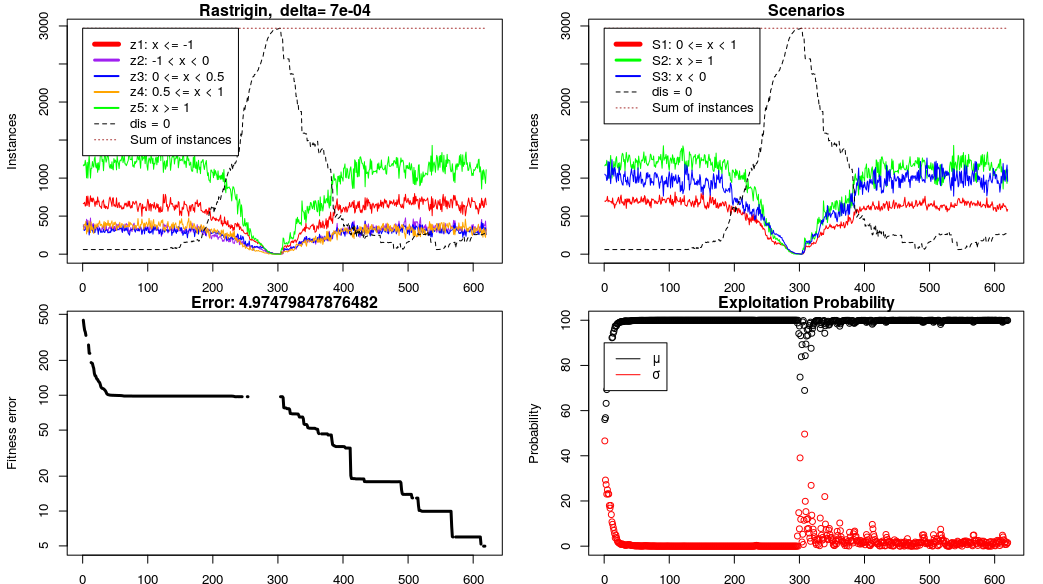
\includegraphics[width=0.9\textwidth]{images/sample.png}
	\caption{My wonderful figure on exploration vs. exploitation. \label{fig:wonderful}}
\end{figure}

Using \LaTeX you can write your equations (see Eq.~\ref{eq:DFO-Update}) and include tables (see Table~\ref{table:Comparison}).

\begin{equation}
	x^{t+1}_{id} = x^t_{i_nd} + u (x_{sd}^t - x_{id}^t) \label{eq:DFO-Update}
\end{equation}

\begin{table}[h]
	\caption{Comparison table} \label{table:Comparison}
	\centering
	\begin{tabular}{lcc}
		\hline
		 & Algorithm 1 & Algorithm 2 \\
		\hline
		\hline
		Problem 1 & 0.89 & 0.65 \\
		Problem 2 & 0.77 & 0.78 \\
		\hline 
	\end{tabular}
\end{table}

\section{Methodology}
Begin writing your methodology here, and state what steps you are going to take in order to accomplish the objectives of your project.

\section{Evaluation}
Begin writing how you intend to evaluate your project in this section.


\bibliographystyle{agsm}
\bibliography{bibliography} %import biblography to be used for references here, replace the bibliography.bib with the name of your .bib file

\end{document} %end the document